\documentclass[titlepage,11pt]{article}

\textwidth 6.5in
\textheight 9in
\oddsidemargin -0.2in
\topmargin -0.5in

\usepackage{indentfirst,graphics,alltt,epsfig,color}

\title{iBioSim: Installation Instructions}

\author{Chris J. Myers}

\date{Created: August 11th, 2008\\
  Last Revised: August 14th, 2008
}

\begin{document}

\maketitle

%show only subsection granularity in the toc
%\setcounter{tocdepth}{2} 
  
\tableofcontents

\clearpage
  
%\setlength{\parindent}{0em}
%\setlength{\parskip}{10pt}

\section{General Requirements}

\noindent
There are versions of {\tt iBioSim} available for Windows, Linux, and
MacOS.  You can download the appropriate installation file from:\\
%%tth:\begin{html}<a href="http://www.async.ece.utah.edu/iBioSim/">\end{html}
{\tt http://www.async.ece.utah.edu/iBioSim}
%%tth:\begin{html}</a>\end{html}
\\ {\tt iBioSim} requires that you have 
%%tth:\begin{html}<a href="http://java.sun.com/javase/downloads/index.jsp">\end{html}
Java Runtime Environment 1.5
%%tth:\begin{html}</a>\end{html}
or higher install on your system.  It also requires that you have 
%%tth:\begin{html}<a href="http://www.graphviz.org/">\end{html}
Graphviz.
%%tth:\begin{html}</a>\end{html}
Also, you should associate files with a ``.dot'' extension with the 
{\tt Graphviz} tool, and files with the ``.xhtml'' extension to your
web browswer.

\section{Installation on Windows}

\noindent
Download and execute {\tt iBioSim-$\langle$version$\rangle$-Setup.exe}.\\
The installation uses InstallJammer.  It first asks you for your
preferred installation language.  Make your selection and press {\tt OK}.

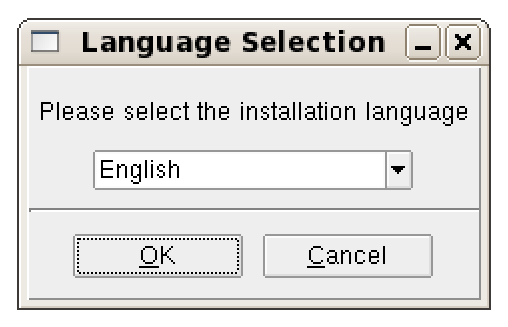
\includegraphics[height=40mm]{screenshots/language}

The next screen tells you that you what version you are installing.
Press {\tt Next} to continue.

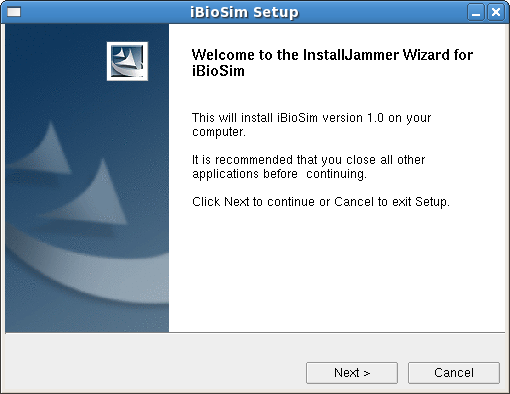
\includegraphics[height=95mm]{screenshots/setup}

\clearpage

Next, it ask you for an installation location.  Please make sure to
select a path that does not have any spaces or special symbols as
these cause problems with {\tt iBioSim}.

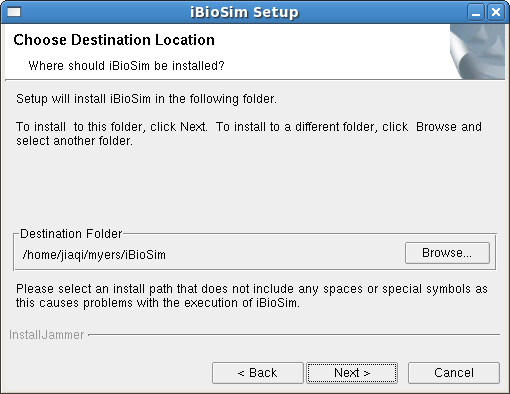
\includegraphics[height=95mm]{screenshots/location}

You are now ready to install.  Press {\tt Next} to continue.

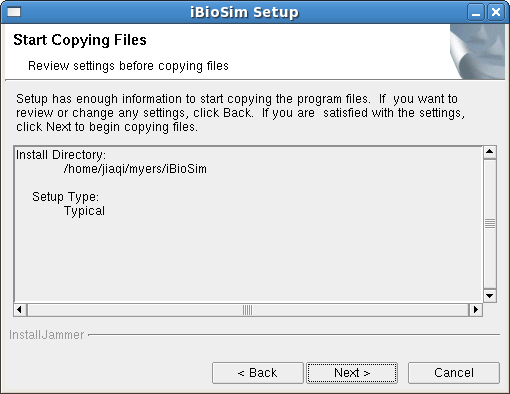
\includegraphics[height=95mm]{screenshots/confirm}

\clearpage

You are all done.  Press {\tt Finish}.  If selected, {\tt iBioSim}
will launch immediately.  Otherwise, you can start it using your
desktop shortcut or from your start menu.

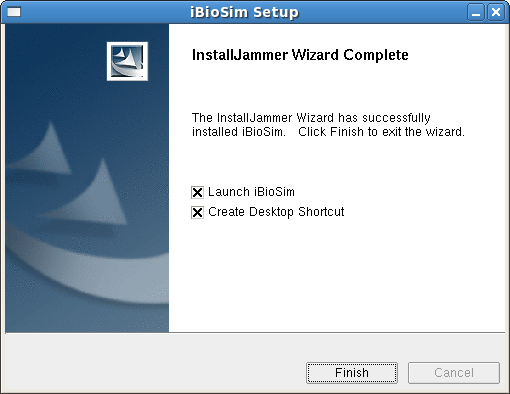
\includegraphics[height=95mm]{screenshots/finish}

In your start menu, there should be an option to uninstall.  If you
select this, it will ask if you are sure then proceed to completely
remove {\tt iBioSim} from your system.  It is highly recommended that
you remove {\tt iBioSim} using this uninstall procedure before
installing a new version.

\section{Installation on Linux}

\noindent
Since InstallJammmer is also used for the Linux install, the
installation instructions are essentially the same.
First, download {\tt iBioSim-$\langle$version$\rangle$-Linux-x86-Install}.
Open a terminal and browse to where this file was download.  You must
make this file executable:\\
{\tt chmod u+x iBioSim-$\langle$version$\rangle$-Linux-x86-Install}.
You should then execute this file:\\
{\tt ./iBioSim-$\langle$version$\rangle$-Linux-x86-Install}.
This starts InstallJammer.  It first asks you for your
preferred installation language.  Make your selection and press {\tt OK}.

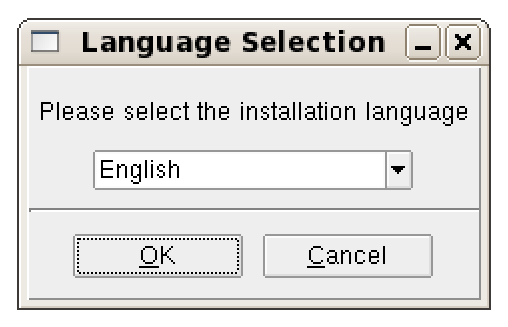
\includegraphics[height=40mm]{screenshots/language}

\clearpage

The next screen tells you that you what version you are installing.
Press {\tt Next} to continue.

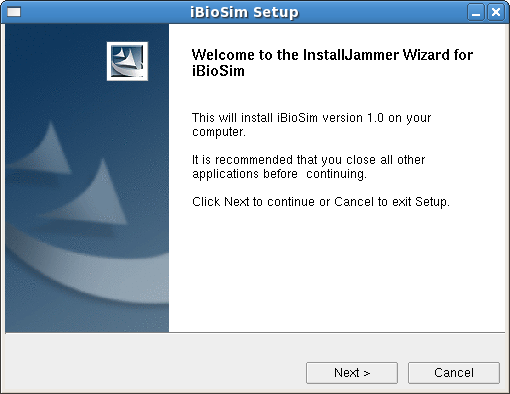
\includegraphics[height=95mm]{screenshots/setup}

Next, it ask you for an installation location.  Please make sure to
select a path that does not have any spaces or special symbols as
these cause problems with {\tt iBioSim}.

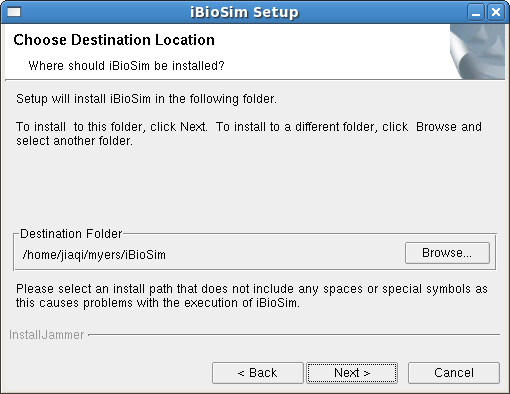
\includegraphics[height=95mm]{screenshots/location}

\clearpage

You are now ready to install.  Press {\tt Next} to continue.

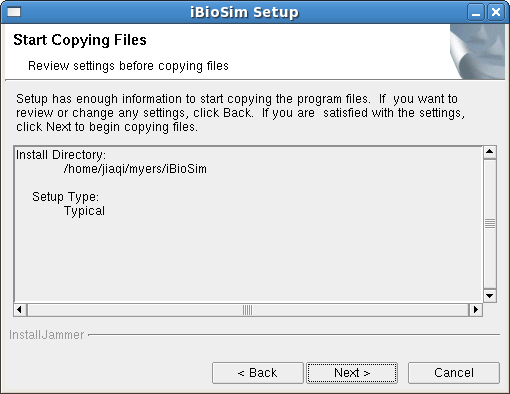
\includegraphics[height=95mm]{screenshots/confirm}

You are all done.  Press {\tt Finish}.  If selected, {\tt iBioSim}
will launch immediately.  Otherwise, you can start it using your
desktop shortcut or from your start menu.

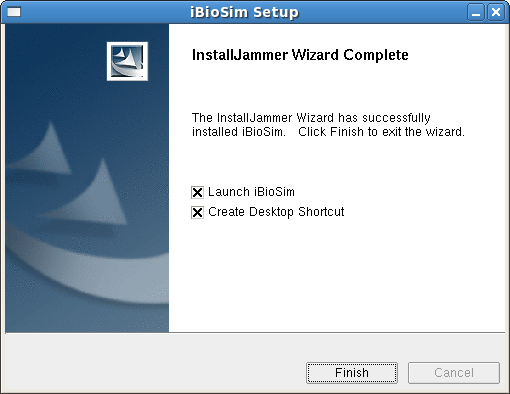
\includegraphics[height=95mm]{screenshots/finish}

In your start menu, there should be an option to uninstall.  If you
select this, it will ask if you are sure then proceed to completely
remove {\tt iBioSim} from your system.  It is highly recommended that
you remove {\tt iBioSim} using this uninstall procedure before
installing a new version.

\clearpage

\section{Installation on MacOS}

\noindent
To install on MacOS, you need to download {\tt iBioSim.dmg}.  You should
open this file with {\tt DiskImageMounter.app}.  This should open up
this disk image in {\tt finder}.  You should then
double-click on the {\tt iBioSim} package.  

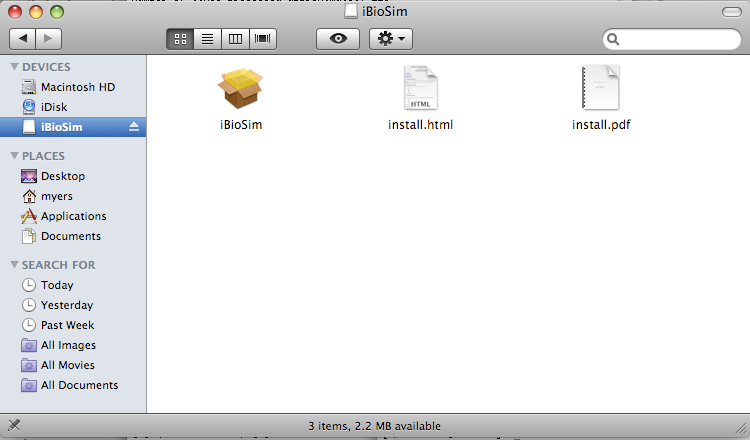
\includegraphics[height=95mm]{screenshots/finder}

This starts the {\tt iBioSim} installer.  Press {\tt Continue} to go on.

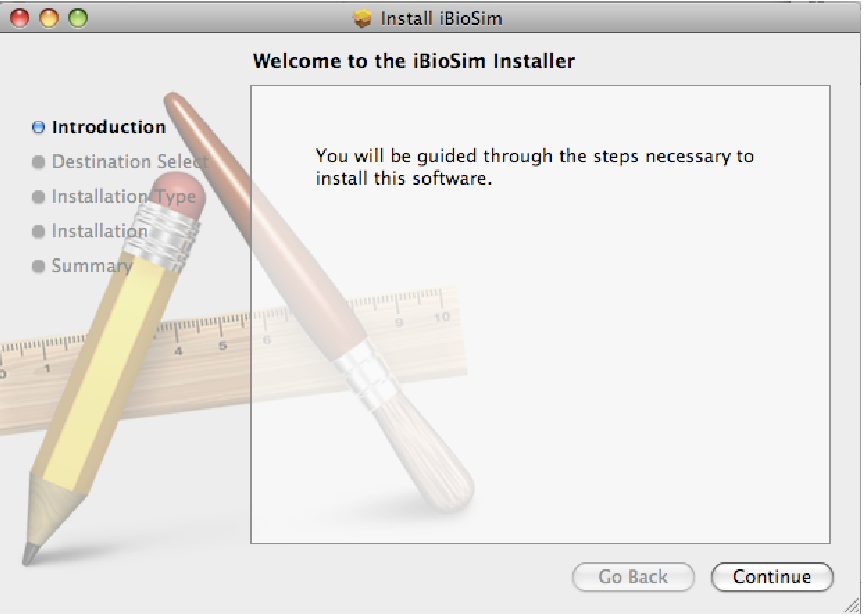
\includegraphics[height=95mm]{screenshots/intro}

\clearpage

You should now select the drive you wish to install on.  {\tt iBioSim}
will be installed in your {\tt Applications} directory on this drive.

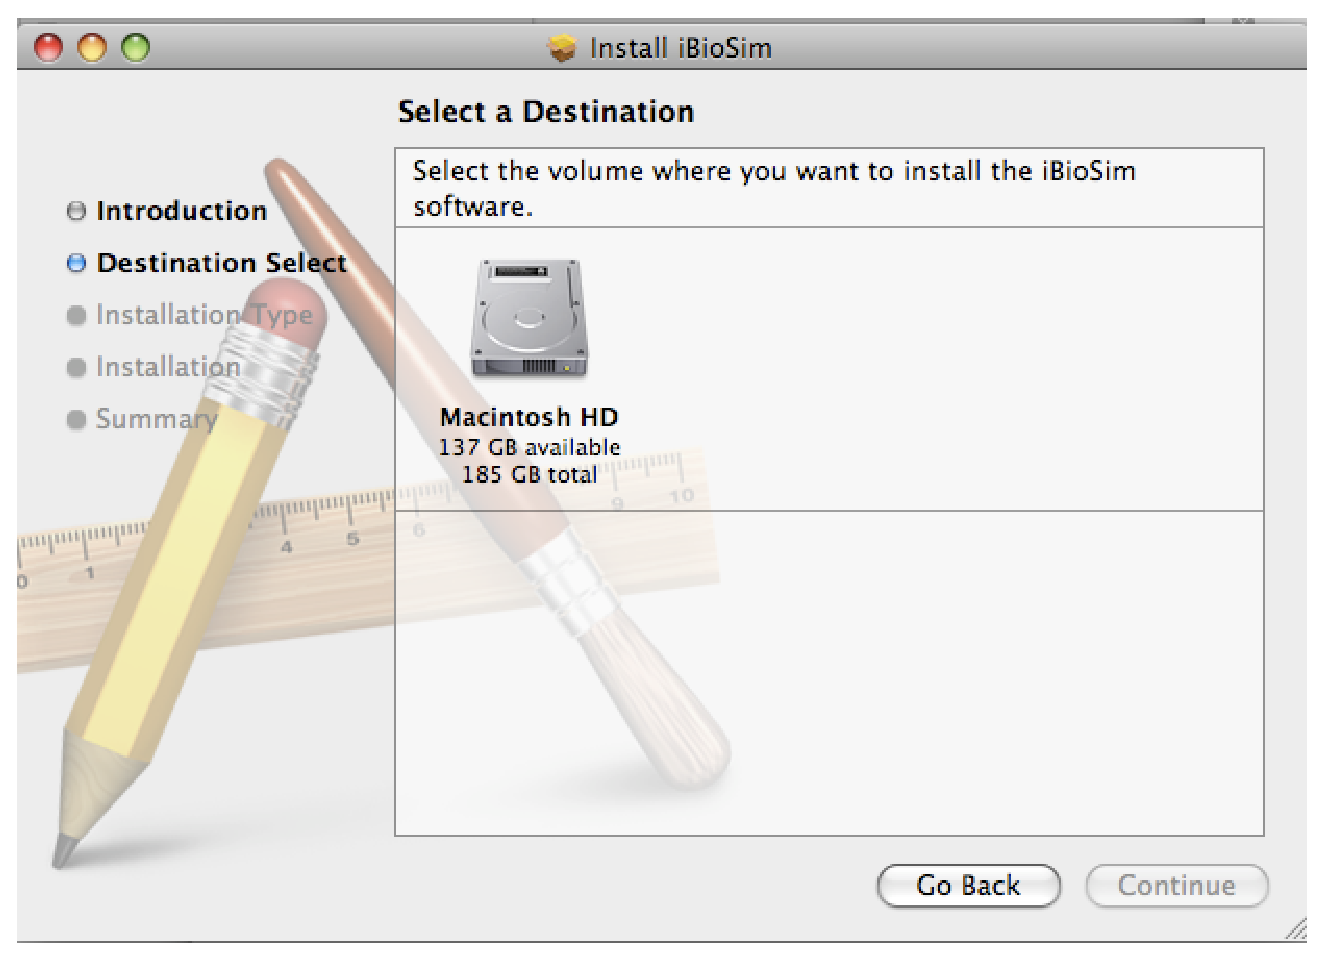
\includegraphics[height=95mm]{screenshots/destination}

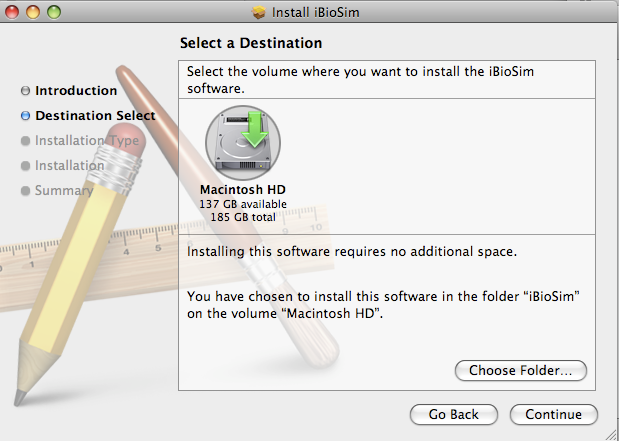
\includegraphics[height=95mm]{screenshots/select}

\clearpage

It will then tell you how much space it will take and allow you to
confirm that you wish to install by pressing {\tt Install}.

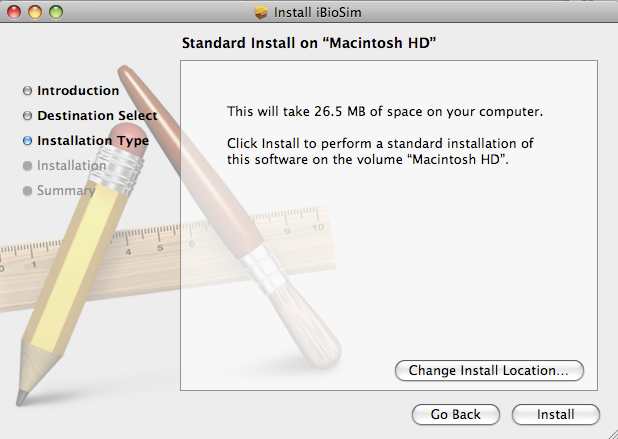
\includegraphics[height=95mm]{screenshots/installType}

You should then get a message that it installed correct.  At this
point, you should be able to use {\tt Finder} and locate {\tt iBioSim}
in your {\tt Applications} directory.  {\tt iBioSim} is started by
double-clicking on it.

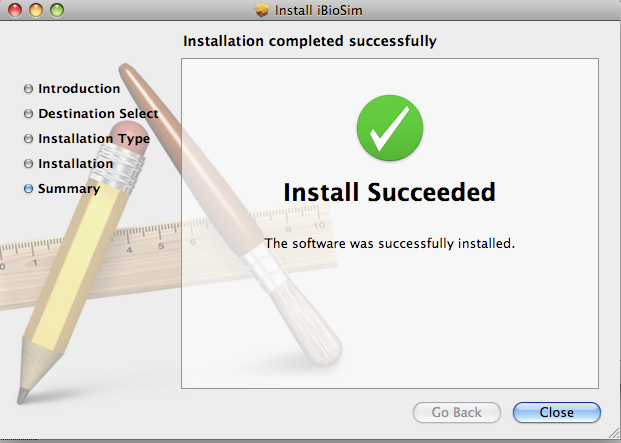
\includegraphics[height=95mm]{screenshots/success}

\end{document}
